\documentclass{beamer}
\usepackage[utf8]{inputenc}
\usepackage[T2A]{fontenc}
\usepackage[russian]{babel}
\usepackage{amsmath, amssymb, amsfonts}
\usepackage{graphicx}
\usepackage{caption}
\usepackage{hyperref}

\DeclareMathOperator*{\argmax}{arg\,max}
\DeclareMathOperator*{\argmin}{arg\,min}
\DeclareMathOperator*{\Argmax}{Arg\,max}
\DeclareMathOperator*{\Argmin}{Arg\,min}

\graphicspath{ {./img/} }

\usetheme{Madrid}
\usecolortheme{default}

\title{Анализ и применение многофакторных моделей динамики лекарственных веществ в медицинских исследованиях}
\author{Лазар В. И.}
\institute{ВМК МГУ}

\begin{document}

\begin{frame}
	\titlepage
\end{frame}

\begin{frame}{Содержание}
	\tableofcontents
\end{frame}

%%%%%%%%%%%%%%%%%%%%%%%%%%%%%%%%%%%%%%%%%%
\section{Введение и постановка задачи}
%%%%%%%%%%%%%%%%%%%%%%%%%%%%%%%%%%%%%%%%%%
\begin{frame}{Введение}
	\begin{itemize}
		\item \textbf{Фармакокинетика (ФК):} исследование ADME лекарственных средств.
		\item Значение многофакторных моделей, учитывающих физиологические, биохимические и генетические факторы.
		\item Проблемы исследований: малые выборки, неравномерность замеров, шум и выбросы.
		\item Актуальность модели \textbf{PBFTPK} для описания межиндивидуальной вариабельности.
	\end{itemize}
\end{frame}

\begin{frame}{Постановка задачи}
	\begin{itemize}
		\item Классические модели PBFTPK описывают одно-пиковые траектории.
		\item Необходимость адаптации моделей для траекторий с несколькими пиками и фазами.
		\item Цель: разработка модифицированной модели, устойчивая к шуму, с корректной оценкой параметров.
		\item Использование методов минимаксного и пикового определения параметров ($\tau$, $\tau_0$).
	\end{itemize}
\end{frame}

%%%%%%%%%%%%%%%%%%%%%%%%%%%%%%%%%%%%%%%%%%
\section{Описание данных и моделей}
%%%%%%%%%%%%%%%%%%%%%%%%%%%%%%%%%%%%%%%%%%
\begin{frame}{Описание данных}
	\begin{itemize}
		\item Данные представлены в виде временных рядов концентрации лекарства.
		\item Особенности: неравномерность замеров, разные порядки измерений, фазовый рост и спад концентрации.
		\item Пример траектории иллюстрирован на графике.
	\end{itemize}
	\begin{center}
		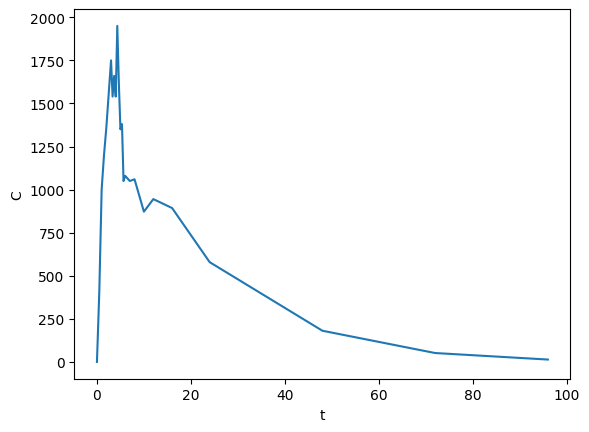
\includegraphics[width=0.6\linewidth]{sample.png}
	\end{center}
\end{frame}

\begin{frame}{Описание моделей: PBFTPK}
	\textbf{PBFTPK\_0:}
	\[
		C(t) =
		\begin{cases}
			\frac{FD}{\tau} \frac{1}{V_d k_{el}} (1 - e^{-k_{el} t}), & t \leq \tau \\
			C(\tau)e^{-k_{el}(t-\tau)},                               & t > \tau
		\end{cases}
	\]
	\vspace{0.5em}
	\textbf{PBFTPK\_1:}
	\[
		C(t) =
		\begin{cases}
			\frac{FD k_a}{V_d (k_a - k_{el})} \Big(e^{-k_{el}t} - e^{-k_a t}\Big), & t \leq \tau \\
			C(\tau)e^{-k_{el}(t-\tau)},                                            & t > \tau
		\end{cases}
	\]
	\begin{itemize}
		\item Параметры: \( F, D, V_d, k_a, k_{el}, \tau \)
	\end{itemize}
\end{frame}

\begin{frame}{Кусочная модификация PBFTPK}
	\begin{itemize}
		\item Введение дополнительных параметров: \( \tau_0 \) и \( \tau_{max} \).
		\item Новая модель (на примере PBFTPK\_1):
		      \[
			      C(t) = \begin{cases}
				      0,                                                             & t \le \tau_0        \\
				      \frac{FD k_a}{V_d (k_a - k_{el})} (e^{-k_{el}t} - e^{-k_a t}), & \tau_0 < t \le \tau \\
				      C(\tau)e^{-k_{el}(t-\tau)},                                    & t > \tau
			      \end{cases}
		      \]
		\item Методы определения \( \tau \) и \( \tau_0 \):
		      \begin{itemize}
			      \item \textbf{Минимаксный метод:}
			            \[
				            \tau = \argmax_{t < \tau_{max}} C(t), \quad \tau_0 = \argmin_{t < \tau} C(t)
			            \]
			      \item \textbf{Пиковый метод:}
			            \[
				            \tau = \max\,\Argmax_{t < \tau_{max}} C(t), \quad \tau_0 = \max\,\Argmin_{t < \tau} C(t)
			            \]
		      \end{itemize}
	\end{itemize}
\end{frame}

\begin{frame}{EPBFTPK и функция потерь}
	\textbf{EPBFTPK:}
	\begin{itemize}
		\item Ансамблирование моделей: построение \(\hat{C}_i(t)\) на основе остатков \(r(t) = C(t) - \hat{C}(t)\).
		\item Итоговая оценка:
		      \[
			      \hat{C}(t) = \sum_i \hat{C}_i(t)
		      \]
	\end{itemize}
	\vspace{0.5em}
	\textbf{Функция потерь:} \(\lambda\)-взвешенная MSE
	\[
		L_{\lambda} = \frac{1}{N}\sum_{i=1}^{N} \Big(C(t_i)-\hat{C}(t_i)\Big)^2 \cdot
		\begin{cases}
			1,       & t_i \le \tau \\
			\lambda, & t_i > \tau
		\end{cases}
	\]
	\begin{itemize}
		\item Регулировка влияния ошибок на фазах абсорбции и элиминации.
	\end{itemize}
\end{frame}

%%%%%%%%%%%%%%%%%%%%%%%%%%%%%%%%%%%%%%%%%%
\section{Итоговый алгоритм и результаты}
%%%%%%%%%%%%%%%%%%%%%%%%%%%%%%%%%%%%%%%%%%
\begin{frame}{Итоговый алгоритм}
	Задача оценки сводится к последовательной минимизации:
	\[
		L_{\lambda}(r_i, \hat{C}_i, t) \to \inf_{p \in \Omega}
	\]
	где
	\[
		\Omega = \{ (F, D, V_d, k_a, k_{el}) \mid F \in [0,1],\, D \ge 0,\, V_d \ge 0,\, k_a \ge 0,\, k_{el} \ge 0 \}
	\]
	\[
		r_1 = C
	\]
	\begin{itemize}
		\item Метод можно адаптировать для предсказания траектории.
	\end{itemize}
\end{frame}

\begin{frame}{Результаты исследований}
	\begin{itemize}
		\item Сравнение моделей: базовая PBFTPK и ансамблированная EPBFTPK.
		\item EPBFTPK демонстрирует лучшую точность, особенно при сложных траекториях с задержанным спадом.
		\item Ошибки максимальны в точках пиков (\(\tau_i\)).
	\end{itemize}
	\begin{center}
		\small
		\textbf{Примеры графиков:}
		\vspace{0.5em}

		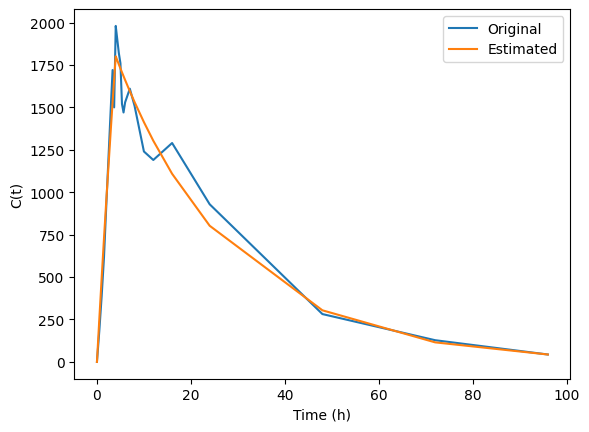
\includegraphics[width=0.4\linewidth]{results/basic_1.png} \quad
		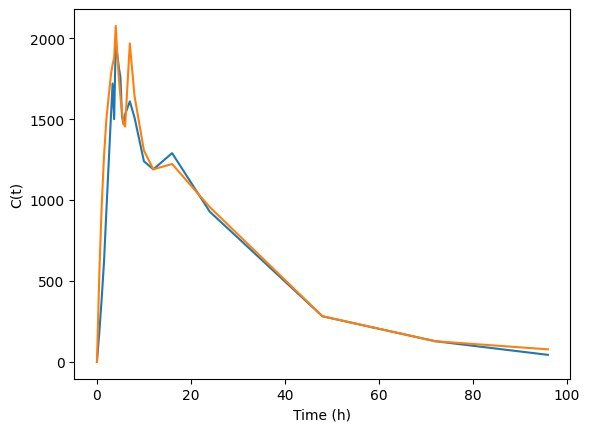
\includegraphics[width=0.4\linewidth]{results/1.jpg}
	\end{center}
\end{frame}

%%%%%%%%%%%%%%%%%%%%%%%%%%%%%%%%%%%%%%%%%%
\section{Заключение}
%%%%%%%%%%%%%%%%%%%%%%%%%%%%%%%%%%%%%%%%%%
\begin{frame}{Выводы}
	\begin{itemize}
		\item Многофакторные модели PBFTPK успешно описывают динамику концентрации лекарственных веществ.
		\item Модификации и ансамблирование (EPBFTPK) позволяют учитывать сложные траектории и улучшать точность модели.
		\item Применение взвешенной функции потерь помогает компенсировать неравномерность данных.
	\end{itemize}
\end{frame}


\end{document}
